\documentclass[12pt,letterpaper]{article}
% Paqueteria Necesaria
\usepackage[utf8]{inputenc}
\usepackage[english, spanish]{babel}
\usepackage[round,sort,numbers]{natbib}
\usepackage[font={small,bf},tableposition=top]{caption}
\usepackage{url}
\usepackage{amsmath}
\usepackage{array}
\usepackage{xcolor, colortbl}
\usepackage{lscape}
\usepackage{amssymb}
\usepackage{makeidx}
\usepackage{enumerate}
\usepackage{graphicx}
\usepackage{fontenc}
\usepackage[T1]{fontenc}
\usepackage{helvet}
\renewcommand*\familydefault{\sfdefault}
\usepackage[left=3cm,right=2cm,top=3cm,bottom=3cm]{geometry}
\usepackage{setspace}
\usepackage{fancyhdr}
\makeatletter
\renewcommand\@biblabel[1]{#1}
\makeatother
% Colores
\definecolor{blanc}{rgb}{.83,.83,.83}
% Interlineado y Salto de linea
\spacing{1.5}
\hyphenation{ge-ne-rán-do-se}
\begin{document}	
	\begin{titlepage}	
	\setlength{\parskip}{1.5cm}
	% Estructura del documento
\begin{titlepage}
% Titulo superior
\begin{center}
	\selectlanguage{english}{
	{\fontsize{18}{1.5}\selectfont \textbf{UNIVERSIDAD DE GUADALAJARA}}
	
	{\fontsize{14}{1.5}\selectfont\textbf{Centro Universitario de Los Lagos}}
	\vspace{1cm}
% Parametros para la imagen de portada
	\begin{figure}[h]
	\centering
	\includegraphics[height=3.57cm,width=3cm]{/home/Fdora/Pictures/UdeG.png}
	\end{figure}
	\\
	\vspace{1cm}
% Titulo inferior
	{\fontsize{14}{1.5}\selectfont \textbf{"Análisis y Modelado de Parámetros Biocinéticos de Lodos Activados Provenientes de la Planta Municipal de Tratamiento de Aguas Residuales de Lagos de Moreno"}}
	
	{\fontsize{14}{1.5}\selectfont Protocolo de Tesis para obtener el Título de Ingeniero Bioquímico}
	
	{\fontsize{14}{1.5}\selectfont Presenta: \\ \textbf{Luis David Rodríguez Centeno}}
	
	{\fontsize{14}{1.5}\selectfont Director de Tesis: \\ \textbf{M. en C. Gabriela Camarillo Martínez}}}
	
	\vfill
% Fecha
	Lagos de Moreno, Jal. \selectlanguage{spanish}{\today}
\end{center}
\end{titlepage}

	\end{titlepage}
	\setcounter{page}{2}
\newpage
 	% Cuerpo del documento
\subsection*{Introducción}
En los últimos años, el correcto uso de los recursos hidráulicos se ha convertido en tema de interés. Esto se debe principalmente a la cada vez más notable escasez de agua potable, tanto por acción del cambio climático como por el creciente uso indiscriminado de este recurso para satisfacer las crecientes necesidades de la población y al prácticamente nulo tratamiento de las aguas residuales \citep{informeods2021, aa2030}.\par
Con base a los datos presentados por el monitor de sequía~\citep{msm}, en los últimos años Lagos de Moreno ha enfrentado problemas de sequía moderada a severa durante la temporada seca, aunado a los crecientes problemas de sobre-explotación de los acuíferos de la cuenca pone en riesgo la sustentabilidad con base a los Objetivos de Desarrollo Sustentable 2030 \citep{aa2030}. De acuerdo a los datos disponibles en el portal de la Comisión Nacional del Agua (Conagua) \citep{acuiferolag} el acuífero cuenta con una capacidad de recarga estimada de 196 Mn$^{3}$/año y un volumen de extracción de aguas subterráneas de 22811730 m$^{3}$ anuales; teniendo como resultado un déficit de 3211730 m$^{3}$ anuales y, por consecuencia, la nula posibilidad de generar nuevas concesiones para la creación de pozos de extracción.\par
Ateniéndonos a los datos presentes en la \emph{Agenda del Agua 2030} \citep{aa2030}, tan solo el 91.3\% de la población cuenta con servicio de agua potable y 89.9\% tiene cobertura de alcantarillado del cual, solo un 43.4\% recibe tratamiento. Las estimaciones esperadas rumbo a 2030 indican que se requerirá infraestructura para dar un tratamiento correcto a 7.157 miles de millones de metros cúbicos, generando una brecha de 4.3 miles de millones de metros cúbicos \citep{aa2030}.\par
La Comisión Estatal del Agua (CEA) que es la institución encargada del vigilar el uso correcto del agua en el estado de Jalisco, mediante la ficha técnica hidrológica del municipio, informa que se cuentan con 3 plantas de tratamiento de aguas residuales  en funcionamiento con capacidad de operación de 114.6 L/s, cubriendo un 33.8\% de saneamiento (datos pertenecientes al 2015) \citep{fichalagos}.\\
En México las principales normas que existen en materia de tratamiento y calidad del agua son la \textbf{NOM-003-ECOL-1997}, la cual determina los límites máximos permisibles de contaminantes presentes en los efluentes de las plantas de tratamiento que sean reusadas; y la reciente \textbf{NOM-001-SEMARNAT-2021} la cual remplaza a la \textbf{NOM-001-ECOL-1996} que establece los límites permisibles de contaminantes en las descargas de aguas residuales sin tratar en cuerpos receptores nacionales.

\subsection*{Antecedentes}
\subsubsection*{Características de las aguas residuales}
Podemos definir a las aguas residuales como aquellas que provienen de las actividades del hombre y de los animales, tanto como de las precipitaciones, y que son recolectadas en los sistemas de alcantarillado o vertidas directamente al ambiente \citep{carreno17}.\\
Los principales ensayos para determinar la carga orgánica de un desagüe son: la demanda bioquímica de oxígeno (DBO) y la demanda química de oxígeno (DQO) \citep{carreno17}.\\
Podemos dividirlas según su origen en seis clases:
\begin{description}
\item[\textit{Aguas residuales domésticas}]
Las aguas residuales domésticas son flujos de agua conformados por la combinación de las excretas eliminadas por la población, que incluye heces y orina; además, contiene desechos de animales domésticos, residuos de lavandería, residuos de industrias caseras que algunas veces vierten sustancias recalcitrantes que pueden ser cancerígenas, y residuos de las actividades culinarias. La gente excreta de 100 a 500 g de heces por día y de 1 a 3 L de orina al día, contribuyendo con una DBO$_{5}$ DE 20 a 45 g por día \citep{carreno17}. 
\item[\textit{Aguas residuales municipales}]
Son aquellas provenientes tanto de los efluentes domésticos como de las pequeñas industrias y otras actividades realizadas en las áreas urbanas (comercios, oficinas, restaurantes, mercados de abasto, etc.) y que incrementan los contaminantes con algunos componentes que pueden resultar indeseables para los tratamientos convencionales \citep{carreno17}.
\item[\textit{Aguas residuales industriales}]
Son aquellas provenientes de las distintas industrias que existen generalmente fuera de las áreas urbanas y que deben tratar sus desagües antes de ser vertidos a los alcantarillados, siguiendo las normas sobre vertidos de descargas industriales, relacionadas principalmente con la carga orgánica (CO), los aceites y grasas, temperatura, pH y sustancias recalcitrantes o xenobióticas \citep{carreno17}.
\item[\textit{Aguas residuales agropecuarias o agroindustriales}]
Se refiere a las escorrentías que provienen de la actividad agrícola y de los mataderos, establos, granjas avícolas, etc., que generan gran cantidad de materia orgánica carbonácea, constituidas por el estiércol y purines de los animales, combinado con residuos tóxicos de los pesticidas y fertilizantes usados en la agricultura. hoy en día se deben considerar también los residuos farmacéuticos usados  en la crianza y engorde de los animales, como vacunas, hormonas, antibióticos y otros de tipo veterinario \citep{carreno17}.
\item[\textit{Aguas pluviales}]
Las aguas provenientes de las lluvias que llegan a las alcantarillas, van a diluir la carga orgánica del desagüe; sin embargo, pueden variar las características del agua como el pH, debido a que muchas de estas aguas de lluvia se convierten en lluvias ácidas antes de llegar al suelo y a las alcantarillas; por otro lado, los caudales del desagüe durante el periodo de lluvias también se incrementan, por lo que es un factor importante que se debe tener en cuenta en los diseños para dichas temporadas \citep{carreno17}.
\end{description}

\subsubsection*{Tratamiento de aguas residuales}
El tratamiento de aguas residuales,es un servicio que consiste en la separación de la carga orgánica que contienen las aguas residuales, eliminando al máximo la cantidad de residuos y contaminantes, siendo algunos de los más importantes los descritos en el Cuadro~\ref{tab:constituyentes} \citep{tratGOB, ron}, de tal forma que reúnan los requisitos de calidad que permiten las normas legales y regulaciones de cada país, con la finalidad de que los estándares de calidad ambiental (\emph{ECA}) permanezcan inalterables en el tiempo, y que la preservación sustentable de los ecosistemas sea posible. Sin embargo, en los países en desarrollo esto no se cumple, por lo que solo un pequeño porcentaje de aguas residuales tienen tratamiento y el resto son vertidas al mar, ríos, suelos, etc., originando riesgos de infecciones gastrointestinales e origen hídrico \citep{carreno17}.\par
	\begin{table}[!ht]
	\begin{small}	
	\caption{Principales constituyentes de interés en el tratamiento de aguas residuales}\label{tab:constituyentes}
	\begin{center}
		\begin{tabular}{ | m{5cm} | m{10cm} | }
		\hline 
		\rowcolor{blanc}
		{\textbf{Constituyentes}} & {\textbf{Razones de interés}}\\ 
		\hline 
		Sólidos suspendidos totales & Formación de depósitos de lodos y condiciones anaerobias\par \\ 
		
		Compuestos orgánicos biodegradables & Agotamiento del oxígeno en fuentes naturales y desarrollo de condiciones sépticas\par \\
		
		Constituyentes inorgánicos disueltos (p.ej. sólidos disueltos totales) & Constituyentes inorgánicos adicionados por el uso. Aplicaciones en el reciclaje y en la reutilización de aguas residuales\par \\
		
		Metales pesados & Constituyentes metálicos adicionados por el uso. Muchos se clasifican como polulantes de prioridad\par \\
		
		Nutrientes & Crecimiento excesivo de la vida acuática indeseable, eutroficación, concentración de nitratos en agua para consumo\par \\
		
		Patógenos & Trasmisión de enfermedades\par \\
		
		Polulantes orgánicos prioritarios & Sospechosos de ser carcinogénicos, mutagénicos, teratogénicos o de toxicidad aguda alta. Muchos de los polulantes prioritarios son resistentes a los métodos de tratamiento convencionales (conocidos como compuestos orgánicos refractarios)\\
		\hline
		\end{tabular}
		{\small{Fuente: Crites y Tchobanoglous (2000)}}
	\end{center}
	\end{small}
	\end{table}
La eficacia de la separación de materiales en las aguas por procesos físicos, tiene solución técnica fácilmente intuible por cualquier técnico, como es el caso de la separación de partículas por tamaños y densidad \citep{manuel13}.\par
El problema de cálculo, diseño y operación, empieza a complicarse en el intento de eliminar las sustancias orgánicas putrescibles, ya disueltas, o en forma coloidal por biodegradación, presentando la mayor dificultad en la etapa de tratamiento secundario, donde se logra hacer desaparecer la contaminación de las aguas \citep{delapena13}.\par
Al reactor biológico llegan las corrientes procedentes de la etapa de tratamiento primario y la de retorno de lodos, a la vez que se suministra oxígeno al sistema mediante aireación. De modo que el sustrato orgánico es biodegradado por los lodos activos, generándose nueva masa de lodos activos. El contenido del reactor biológico fluye al sedimentador secundario, también llamado clarificador final, en donde se separa una corriente superior clarificada, que pasa a tratamiento terciario. la corriente inferior del sedimentador, constituida por lodos activos concentrados, retorna \emph{Q$_{r}$} en su mayor parte del reactor biológico, y una pequeña fracción \emph{Q$_{w}$} se lleva fuera de esta etapa para su tratamiento específico posterior (\emph{ver} Figura~\ref{fig:balance}) \citep{manuel13}.\par
	\begin{figure}[!h]
		\centering
		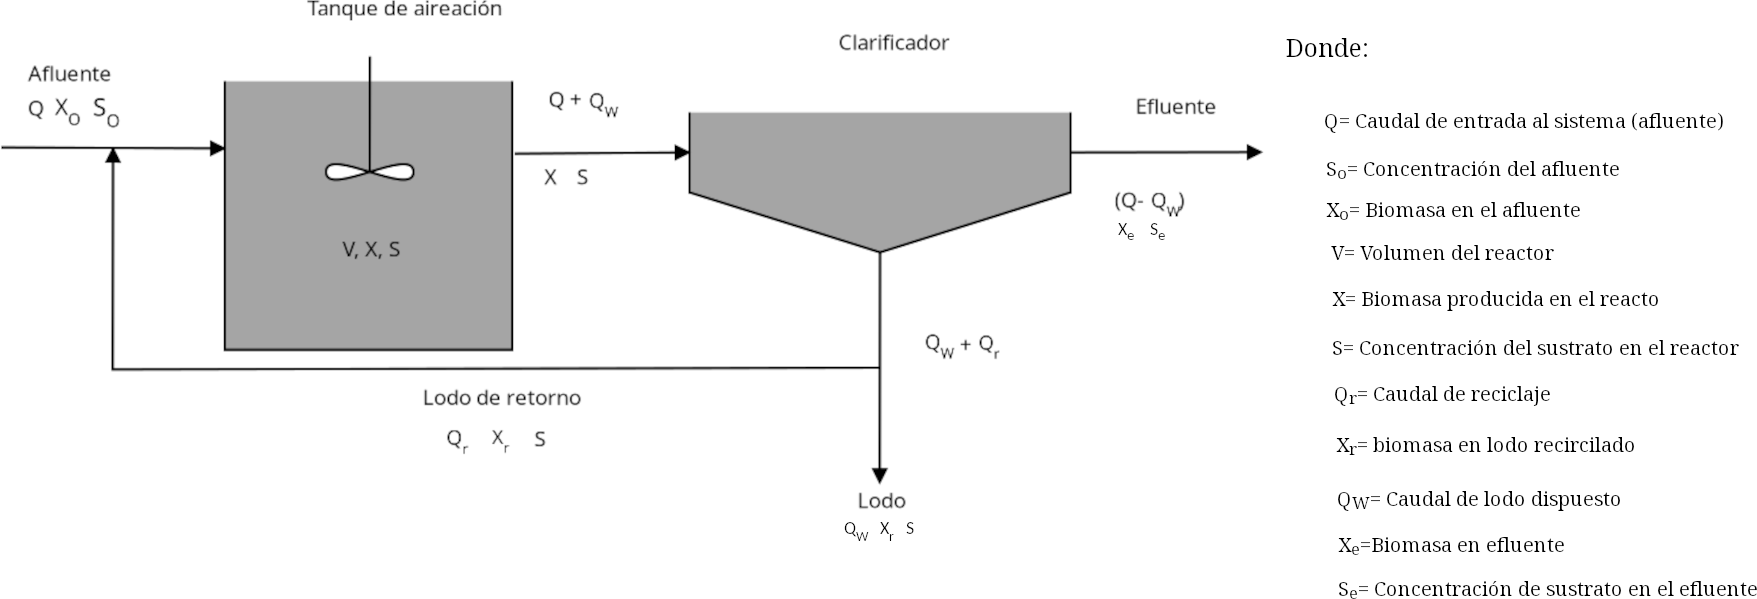
\includegraphics[scale=0.35]{Diagrama_de_flujo.png}
		\caption{Tratamiento secundario de Aguas Residuales}
		\small{Fuente: Elaboración propia}
		\label{fig:balance}
	\end{figure}
El resto de los sólidos sedimentados se recoge como residuo y se desecha. Para que el proceso de oxidación sea eficaz, los microorganismos deben disponer de los niveles adecuados de nutrientes (nitrógeno y fósforo) para la producción de biomasa~\citep{ashok16}.
La temperatura, el pH y el potencial de óxido-reducción son otros de los factores que juegan un papel importante si se busca que el proceso de lodos activos se lleve a cabo de manera efectiva. El rango optimo de pH se encuentra entre 6.5 y 9.0; si el pH esta por debajo de 6.5 los hongos podrían por sustrato por encima de las poblaciones bacterianas. El rol que tienen las bacterias en el proceso de lodos activos se muestra de manera detallada en la Figura~\ref{fig:rolbacteria}~\citep{ashok16, winkler96}
	\begin{figure}[h]
		\centering
		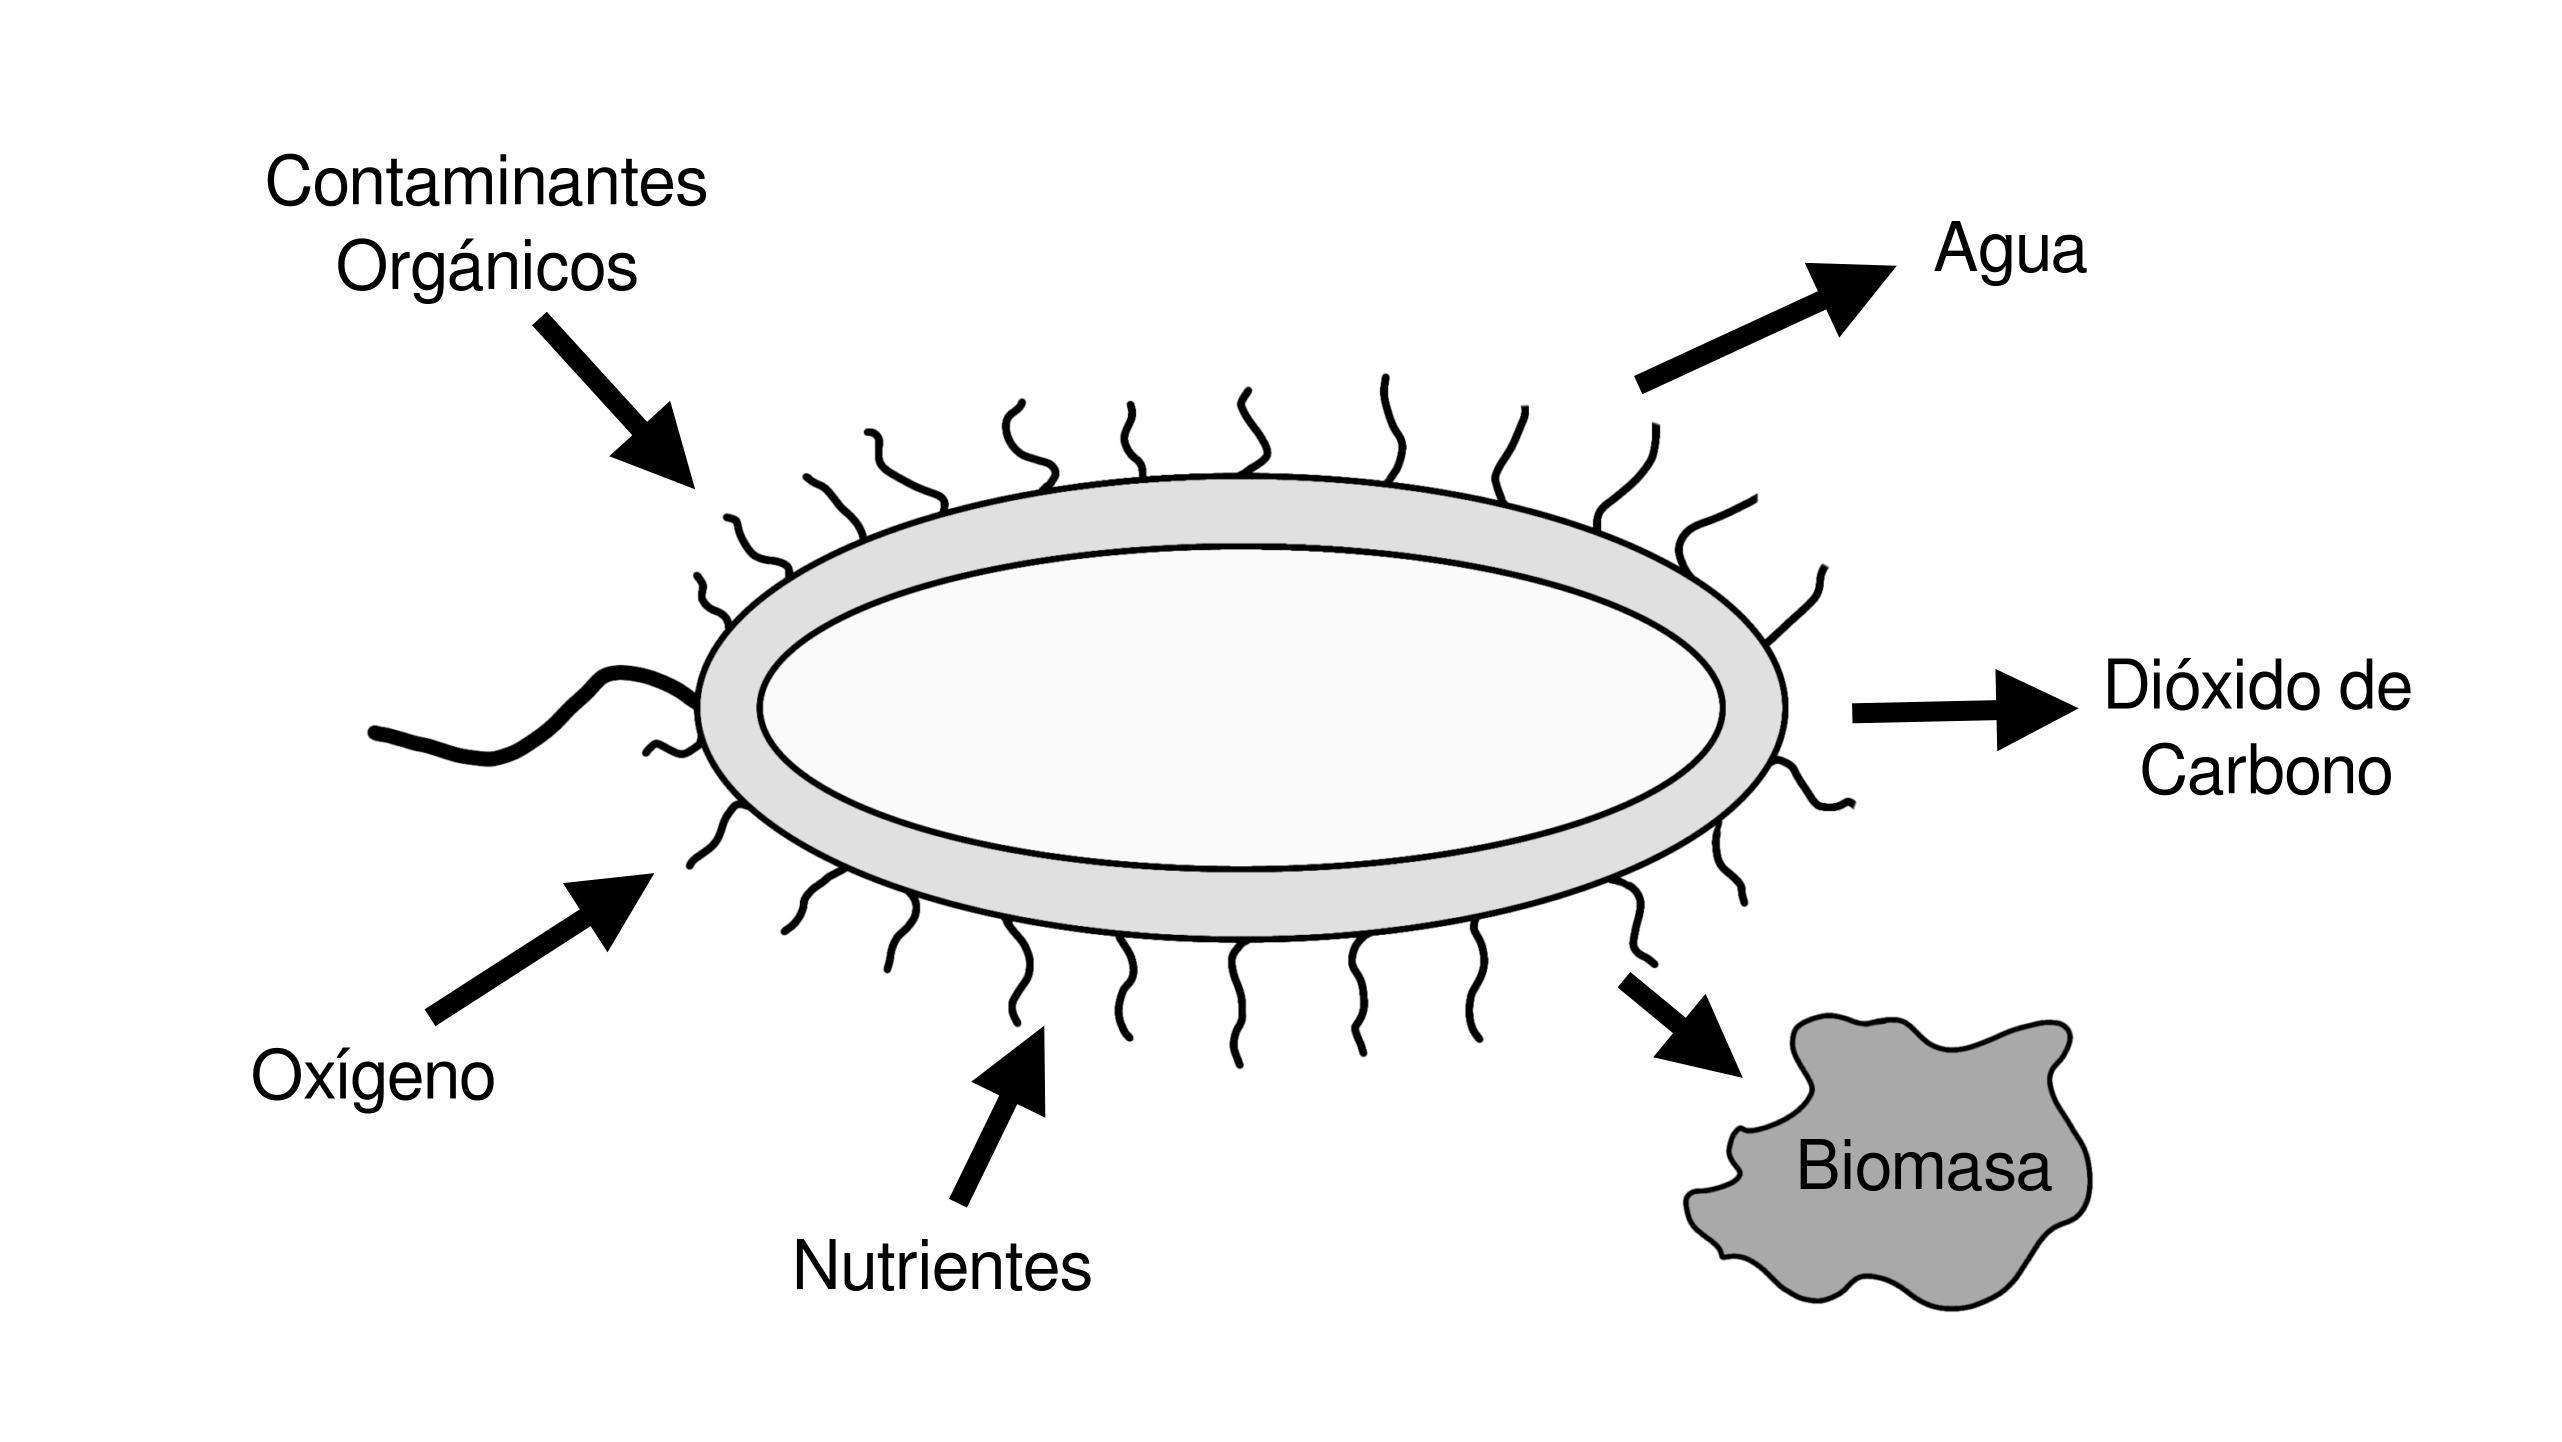
\includegraphics[height=4.5cm,width=10cm]{Bacteria_rol.png}
		\caption{Proceso metabólico bacteriano durante el proceso de lodos activados}
		\small{Fuente: Rathoure (2016)}
		\label{fig:rolbacteria}
	\end{figure}

\subsubsection*{Lodos activados}
El tratamiento con lodos activados es un proceso de tratamiento biológico que involucra cultivo en suspensión de microorganismos aeróbicos con el fin de degradar los contaminantes presentes en el afluente. El cultivo se lleva a cabo en condiciones de mezclado tanto por movimiento mecánico, utilizando propelas y difusores; como por el uso de aereadores que permitan la unión de todos los componentes del caldo de cultivo. Una serie de reacciones bioquímicas tienen lugar en los tanques de aireación, en las cuales se degradan los componentes orgánicos para generar nuevos componentes celulares \citep{ashok16}.\par
	\begin{figure}[h]
		\centering
		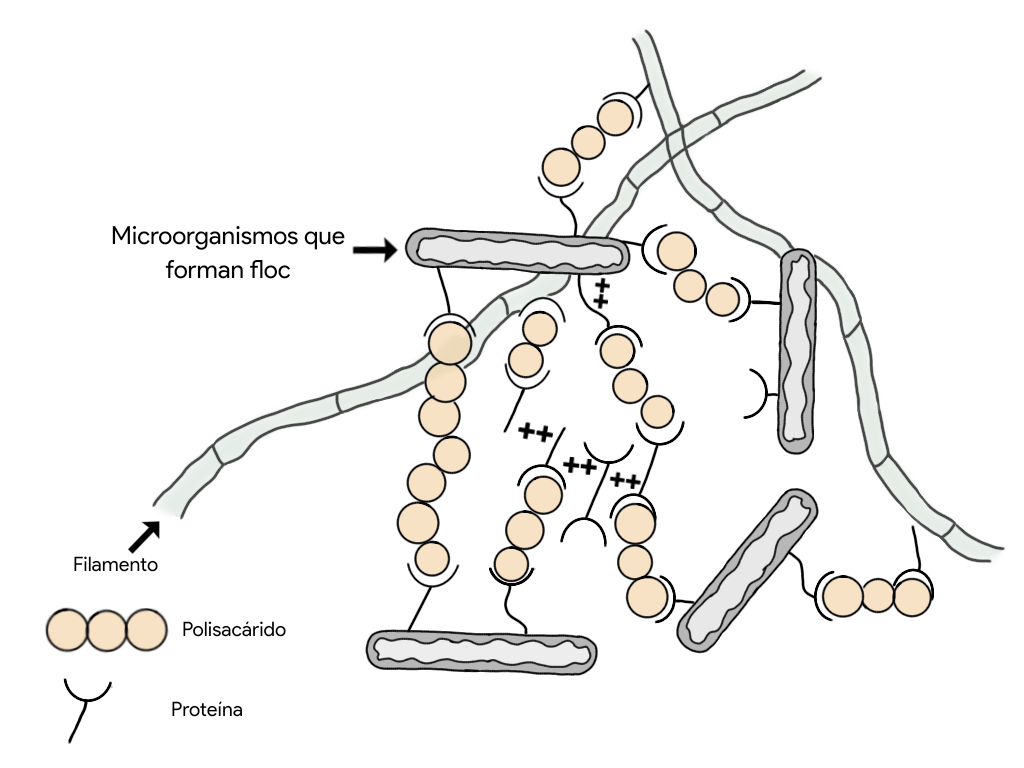
\includegraphics[scale=0.25]{Floculo.png}
		\caption{Modelo de formación de los flocs en lodos activados propuesto por Higgins (1997)}
		\small{Fuente: Elaboración propia}
		\label{fig:modfloc}
	\end{figure}
La unidad ecológica de los lodos es el flóculo individual. Los flóculos de los lodos son cúmulos de varios millones de células bacterianas (principalmente cepas gram-negativas), junto con algunos otros organismos como: hongos, protozoos, rotíferos y nematodos; y materias inertes, orgánicas e inorgánicas (Figura~\ref{fig:modfloc}). La naturaleza floculenta de los lodos activados resulta importante, en primer lugar para la absorción de las materias coloidales, iónicas y en suspensión dentro del agua residual, y en segundo lugar para la separación rápida, eficiente y económica de la masa microbiana del agua residual tratada~\citep{ashok16}. Al airear un agua residual que contenga nutrientes orgánicos tenderá a desarrollar un lodo procedente de los microorganismos ya presentes en ella, o que han entrada de la atmósfera. El proceso de desarrollo de los lodos se puede acelerar por una siembra con una población microbiana, como lodos procedentes de otro proceso, tierras, o en el caso de un desecho industrial que contenga nutrientes fuera de lo común, un cultivo especialmente desarrollado en el laboratorio o una planta piloto~\citep{winkler96}.
Con el paso de los años se han desarrollado variaciones del proceso de lodos activados. Los procesos principales de lodos activados se pueden clasificar como lo muestra la Figura~\ref{fig:procesosaer}.\\
	\begin{figure}[!h]
		\centering
		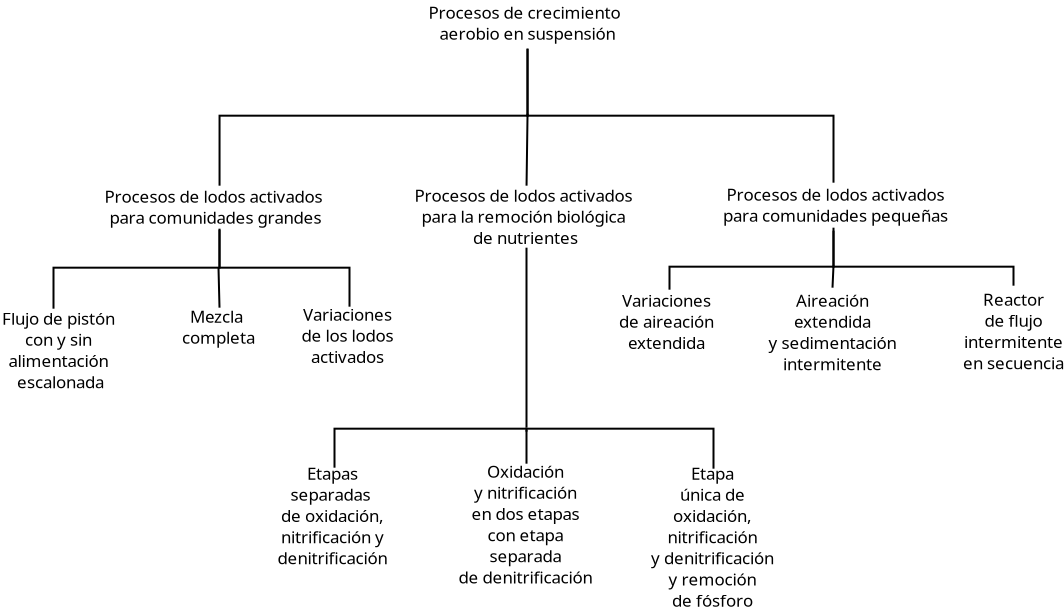
\includegraphics[scale=0.25]{Clasificacion_procesos_aer.png}
		\caption{Esquema de clasificación de los procesos de lodos activados}
		\small{Fuente: Crites (2000)}
		\label{fig:procesosaer}
	\end{figure}
Es importante señalar que los lodos biológicos deben sedimentar adecuadamente, con la finalidad de tener una buena clarificación del agua residual tratada, por lo que es necesario evaluar las características de sedimentación utilizando los siguientes parámetros:
\begin{small}
\begin{enumerate}[a)]
	\item Velocidad de sedimentación zonal (\textbf{VSZ}): depende de la concentración de los lodos.
	\item Índice volumétrico de lodos (\textbf{IVL}): El índice volumétrico de lodos se define como el volumen, en mL, ocupado por 1 g de sólidos suspendidos totales en la muestra, expresados como peso seco, después de sedimentar durante 30 min, en una probeta de 1 L.
\end{enumerate}
\end{small}

\subsubsection*{Oxígeno disuelto}
La cantidad de oxígeno presente en las plantas de tratamiento de aguas residuales (PTAR) determina sus condiciones aerobias, microaerófias, anóxicas y anaerobias para los procesos biológicos. Los desagües crudos, generalmente tienen bajas concentraciones de OD, mientras que los desagües sépticos son anaeróbicos; para los procesos de desnitrificación es necesario un ambiente anóxico, es decir no necesariamente anaeróbico estricto; mientras que en los tanques de aireación de lodos activados y las lagunas aireadas es necesaria la incorporación de oxígeno al sistema\citep{carreno17}.\par
Las PTAR deben monitorearse continuamente para determinar el OD, colocando sondas de oxígeno que permitan su determinación; las lagunas aireadas, igualmente se monitorean a fin de controlar la dotación de oxígeno mediante rotores eléctricos que disminuyen el consumo  de electricidad.

\subsubsection*{Demanda bioquímica de oxígeno}
Se define como la cantidad de OD consumido por los microorganismos para la oxidación de la materia orgánica carbonácea (DBO carbonácea: DBO). Puede considerarse como un procedimiento en el cual los organismos vivos sirven como medio para la oxidación de la materia orgánica hasta dióxido de carbono y agua~\citep{carreno17}.\par
Las reacciones bioquímicas de esta actividad metabólica se resumen en reacciones de síntesis de nuevos organismos, reacciones de producción de energía, para desarrollo de su actividad y reacciones de degradación de los propios microorganismos, consumiendo estas tres reacciones oxígeno, hasta que el sustrato disponible se agota, comenzando entonces la fase de metabolismo endógeno, caracterizado por un consumo mínimo de oxígeno. la DBO mide el consumo de oxígeno en una muestra causado por las reacciones indicadas (\emph{ver} Figura~\ref{fig:estabilizacion})~\citep{manuel13}.

\subsubsection*{Demanda química de oxígeno}
La Demanda Química de Oxígeno, DQO, es el indice general de contaminación más usado. Para aguas blancas, alternativamente se utiliza en lugar de la demanda química de oxígeno, la oxidabilidad al permanganato. En algunas aguas residuales la oxidabilidad al permanganato suministra valores numéricos sensiblemente inferiores a la DQO~\citep{manuel13}.\\
\begin{table}[!h]
\begin{center}
\caption{Comparacion de relaciones de varios parámetros utilizados para caracterizar aguas residuales}
\label{tab:comparacion}
	\begin{tabular}{ | c  c  c |}
	\hline
	\textbf{Tipo de agua residual} & DBO$_{5}$/DQO & DBO$_{5}$/COT \\
	\hline
	No tratada & 0.3-0.8 & 1.2-2.0 \\
	Después de sedimentación primaria & 0.4-0.6 & 0.8-1.2 \\
	Efluente final & 0.1-0.3 & 0.2-0.5 \\
	\hline
	\end{tabular}
	\\{\small{Fuente: Crites y Tchobanoglous 2000}}
\end{center}
\end{table}

Desde el punto de vista operacional, una de las principales ventajas de la prueba de la DQO estriba en que se puede completar en dos horas y media (comparado con los cinco días o más empleados para la prueba de la DBO)~\citep{ron}.
Los valores de la relación DBO$_{5}$/DQO en aguas residuales municipales no tratadas oscilan 0.3 y 0.8. Si la relación DBO$_{5}$/DQO para las aguas residuales no tratadas es mayor que 0.5, los residuos se consideran fácilmente tratables mediante procesos biológicos. Si la relación DBO$_{5}$/DQO es menor de 0.3, el residuo puede contener constituyentes tóxicos o se pueden requerir mocroorganismos aclimatados para su estabilización. La relación DBO$_{5}$/DQO para aguas residuales no tratadas varía de 1.2 a 2.0. Al usar estas relaciones, se debe recordar que ellas cambiarán significativamente de acuerdo con el tratamiento que se haya realizado a los residuos como se muestra en el Cuadro~\ref{tab:comparacion}~\citep{ron}.

\subsubsection*{Parámetros de crecimiento de lodos}
Los parámetros biocinéticos manifiestan el comportamiento de los lodos activados al desarrollarse en determinada agua residual. con base a estos, se pueden obtener por ejemplo: la carga de oxígeno (kg/d) que los lodos biológicos requieren para oxidar la materia orgánica presente; los kilogramos de lodos producidos por la oxidación de la materia orgánica contaminante; las constantes de velocidad;de remoción de contaminantes; de crecimiento; igualmente, a partir de esos parámetros, podemos conocer otros datos importantes con relación a la ingeniería básica del sistema de tratamiento. como lo son: los tiempos de residencia en el biorreactor; el volumen del biorreactor; l capacidad del sistema de aireación; la recirculación de lodos al biorreactor; la carga de lodos que es preciso desechar, etc \citep{martinez2005}.
	\begin{figure}[!h]
		\begin{center}
		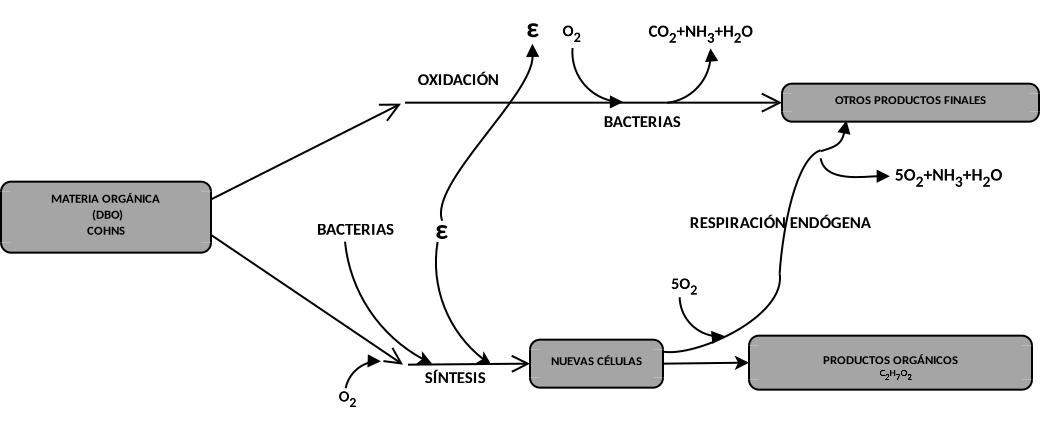
\includegraphics[scale=0.32]{Estabilizacion_mat_org.png}
		\caption{Estabilización de la materia orgánica (DBO) con formación de células nuevas y productos finales}
		\small{Fuente: Crites (2000)}
		\label{fig:estabilizacion}
		\end{center}
	\end{figure}
\\Los microorganismos degradan la materia orgánica soluble en el agua residual siguiendo una cinética específica de remoción de materia orgánica, expresada como remoción de la DBO soluble (\emph{véase} Figura~\ref{fig:estabilizacion}); otras veces puede expresarse como DQO soluble. Entre los modelos más comunes de cinética de remoción de DBO soluble, se encuentran el modelo de \textbf{primer orden}, el de \textbf{orden variable} o \textbf{Monod}, y el de \textbf{Grau}. Los datos experimentales que se obtengan, se utilizan para ajustar un modelo de cinética de remoción, que puede estar entre los anteriormente señalados; de no ser así, se tendrá que probar con otros reportados en bibliografía; incluso, podría ser necesario generar un modelo propio~\citep{martinez2005}.\\
La obtención de los parámetros biocinéticos se basa en la suposición de que el reactor está completamente mezclado y no se tienen limitaciones en la actividad de los lodos activados por oxidación o algún nutriente (nitrógeno y fósforo)~\citep{martinez2005}. Por otra parte, los parámetros se definen como sigue:
	\begin{small}	
	\begin{enumerate}[·]
	\item \textbf{k} = constante especifica de velocidad de remoción de sustrato (d$^{-1}$L/mg). Cinética de primer orden
	\item \textbf{Ks} = constante de afinidad (mg/L). Cinética de orden variable o Monod
	\item \textbf{q$_{max}$} = constante de velocidad especifica máxima de consumo de sustrato(h$^{-1}$). Cinética de orden variable o Monod
	\item \textbf{$\mu_{max}$} = constante de velocidad especifica de crecimiento (h$^{-1}$)
	\item \textbf{Y} (rendimiento) = producción de lodo biológico / Kg de DBO removida (Kg (SSV)/Kg DBOr)
	\item \textbf{a} = Kg de O$_{2}$ (en la oxidación del sustrato) / Kg de DBO removida
	\item \textbf{b} = Kg de O$_{2}$ (para la respiración endógena) /día Kg (SSV) en el reactor
	\item \textbf{kd} (constante de decaimiento o muerte) = Kg de (SSV) (oxidados por respiración endógena) / día Kg (SSV) en el reactor
	\end{enumerate}
	\end{small}

\subsection*{Planteamiento del problema}

\subsection*{Justificación}

\subsection*{Hipótesis}

\subsection*{Objetivos}
\subsubsection*{Objetivo General}

\subsubsection*{Objetivos particulares}

\subsection*{Metodología}

\subsection*{Cronograma}

\bibliographystyle{plain} 
\bibliography{Bibliografia}

\end{document}
 
